\documentclass[letterpaper,mathserif,english,xcolor=dvipsnames]{beamer}

%\usepackage{beamerthemesplit}

\usetheme{Madrid}
%\usecolortheme{beaver}


\usepackage{times}
\usepackage[T1]{fontenc}
\usepackage[latin1]{inputenc}
\usepackage{amsmath}
\usepackage{color}
\usepackage{graphicx}
\usepackage{amssymb}
\usepackage[all]{xy}
\usepackage{tikz}
\usepackage{caption}
\usepackage{subcaption}
\usepackage{tabto}
%\usepackage{bbold}
%\usepackage{animate}

\usepackage{fp}

\theoremstyle{definition}
%\newtheorem{definition}[definition]{Definition}
\theoremstyle{theorem}
%\newtheorem{fact}[theorem]{Fact}
\newtheorem{question}[theorem]{Question}
\newtheorem{ifact}[theorem]{Important Theorem}
\newtheorem{strategy}[theorem]{Strategy}
\newtheorem{proposition}[theorem]{Proposition}
\newtheorem{idea}[theorem]{Idea}
\newtheorem{conjecture}[theorem]{Conjecture}
\newtheorem{dream}[theorem]{Dream}

%\newtheorem{lemma}[theorem]{Lemma}

\newcommand{\R}{\mathbb{R}}
\newcommand{\N}{\mathbb{N}}
\newcommand{\Z}{\mathbb{Z}}
\newcommand{\C}{\mathbb{C}}
\newcommand{\Q}{\mathbb{Q}}
\newcommand{\G}{\mathbb{G}}
%\newcommand{\L}{\mathbb{L}}
\newcommand{\D}{\mathbb{D}}
\newcommand{\A}{\mathbb{A}}
%\newcommand{\P}{\mathbb{P}}
\newcommand{\B}{\mathbb{B}}
\newcommand{\Hidden}[1]{}
\newcommand{\RS}{\mathcal R_S}

\newcommand{\disp}{\displaystyle}

\newcommand{\defbold}[1]{\textcolor{blue}{\textbf{#1}}}
\newcommand{\bigzero}{\mbox{\normalfont\Large 0}}

\DeclareMathOperator{\pr}{pr}
\DeclareMathOperator{\vol}{vol}

\beamertemplatenavigationsymbolsempty

\title[Non-Backtracking Random Walks]{Non-backtracking Random Walks}



\author[Cory Glover]{{\large Cory Glover} \\  \vspace{.2cm}
Brigham Young University \\ Department of Mathematics \\ \vspace{.4cm} {\footnotesize Joint work with\\ Mark Kempton, Brigham Young University\\Tyler Jones, Brigham Young University}
 } \institute[BYU]


\date[February 29, 2020

]{SCR 2020\\Provo, UT\\February 29,2020
}


% Define style for nodes
%\tikzstyle{every node}=[circle, fill=black!50,
%                        inner sep=0pt, minimum width=2pt]
                   
%\tikzstyle{every node}=[circle, draw, fill=black!50,
 %                       inner sep=0pt, minimum width=2pt]
\tikzstyle{every node}=[circle,fill=black,inner sep=1pt]


\newcommand{\F}{\mathbb{F}}


\begin{document}

\frame{\titlepage}



%\section[Outline]{}
%\frame{\tableofcontents}
\colorlet{nodecolor}{red}

%\tikzstyle{every node}=[fill=white,
%                        inner sep=0pt, minimum width=4pt]


%\section{Background}
%\subsection{Original Question}
%\subsection{New Question}

\frame{\frametitle{Problem}

\begin{itemize}
\item When the Pagerank vector of a non-backtracking random walk give the same values as a simple random walk?
\item Can the Pagerank vector of a non-backtracking random walk be calculated faster than a simple random walk?
\end{itemize}

}

\frame{\frametitle{Review}

\begin{definition}[Hashimoto Matrix]
\[B((u,v),(x,y))=\begin{cases}1&v=x,u\neq y\\0&\text{otherwise}\end{cases}\]
\end{definition}

\bigskip

\begin{tikzpicture}
\draw (0,0)node[fill=none]{};
\draw (5,0)node (2)[fill=black]{}--(6,1)node (1)[fill=black]{};
\draw (7,0)node (3)[fill=black]{}--(1);
\draw (4.8,0)node[fill=none]{$u$};
\draw (6.2,1)node[fill=none]{$v$};
\draw (7.2,0)node[fill=none]{$w$};
\path[color=red,every node/.style={font=\sffamily\small}]
    (6,1) edge [->,>=stealth,bend right,shorten >= 1mm,shorten <= 1mm] node [left] {}  (5,0);
\path[color=red,every node/.style={font=\sffamily\small}]
    (6,1) edge [<-,>=stealth,bend left,shorten >= 1mm,shorten <= 1mm] node [right] {}  (5,0);
    \path[color=red,every node/.style={font=\sffamily\small}]
    (6,1) edge [->,>=stealth,bend left,shorten >= 1mm,shorten <= 2.5mm] node [right] {}  (7,0);
    \path[color=red,every node/.style={font=\sffamily\small}]
    (6,1) edge [<-,>=stealth,bend right,shorten >= 1mm,shorten <= 1mm] node [left] {}  (7,0);
\end{tikzpicture}

%\bigskip
%
%Non-backtracking Pagerank (Arrigo et. al, 2018):
%\[(I-\alpha\hat{D}^{-1}B)\hat{y}=\frac{1-\alpha}{n}T^T\hat{D}^{-1}\mathbf{1}\]

}

%\frame{\frametitle{NBRW vs SRW Pagerank}
%
%\begin{itemize}
%\item Ranking (Kendall-Tau Correlation)
%\begin{itemize}
%\item $K(\tau_1,\tau_2)=|\{(i,j)\colon i<j,(\tau_1(i)<\tau_1(j)\wedge\tau_2(i)>\tau_2(j))\vee(\tau_1(i)>\tau_1(j)\wedge\tau_2(i)<\tau_2(j))\}|$
%\end{itemize}
%\item Values (Normed Error)
%\begin{itemize}
%\item $\epsilon=\|\tau_1(i)-\tau_2(i)\|$
%\end{itemize}
%\end{itemize}
%
%}

\frame{\frametitle{Regular Graphs}

\begin{theorem}[Arrigo et. al., 2018]
Let $A$ be the adjacency matrix of an undirected $k$-regular graph, with $k\geq 2$. For any $\epsilon\in[0,1]$, define \[\hat{P}=\epsilon \hat{D}^{-1}B+\frac{1-\epsilon}{n}\mathbf{1}\mathbf{v}^T\] and $P=\epsilon D^{-1}A+\frac{1-\epsilon}{n}\mathbf{1}\mathbf{1}^T$, where $\mathbf{v}=T^TD^{-1}\mathbf{1}$. If $\hat{P}^T\hat{y}=\hat{y}$ and $P^Tx=x$, with $\|x\|_1=\|\hat{y}\|_1=1$, then
\[T\hat{y}=x.\]
\end{theorem}

}

\frame{\frametitle{Bipartite Graphs}

\begin{theorem}
Let $A$ be the adjacency matrix of a bipartite biregular graph, with $d_1,d_2\geq 2$. 
For any $\epsilon\in[0,1]$, define $\hat{P}=\epsilon \hat{D}^{-1}B+\frac{1-\epsilon}{n}\mathbf{1}\mathbf{v}^T$ and $P=\epsilon D^{-1}A+\frac{1-\epsilon}{n}\mathbf{1}\mathbf{1}^T$, where $\mathbf{v}=T^TD^{-1}\mathbf{1}$. If $\hat{P}^T\hat{y}=\hat{y}$ and $P^Tx=x$, with $\|x\|_1=\|\hat{y}\|_1=1$, then
\[T\hat{y}=x.\]
\end{theorem}

}

%\frame{\frametitle{Bipartite Graphs}
%
%\begin{align*}
%B&=\begin{pmatrix}0&B_2\\B_1&0\end{pmatrix}
%\end{align*}
%\smallskip
%\begin{align*}
%T&=\begin{pmatrix}T_1&0\\0&T_2\end{pmatrix}\end{align*}
%\smallskip
%\begin{align*}
%\hat{D}^{-1}&=\begin{pmatrix}\frac{1}{d_2-1}&0\\0&\frac{1}{d_1-1}\end{pmatrix}
%\end{align*}
%\smallskip
%\begin{align*}
%TT^T&=\begin{pmatrix}d_1&0\\0&d_2\end{pmatrix}
%\end{align*}
%
%}

%\frame{\frametitle{Bipartite Graphs}
%
%\textbf{Proof}:
%
%\smallskip
%Recall the equation
%\[(I-\alpha\hat{D}^{-1}B)\hat{y}=\frac{1-\alpha}{n}T^T\hat{D}^{-1}\mathbf{1}.\]
%Since $\alpha\in(0,1)$,
%\begin{align}
%\hat{y}&=\frac{1-\alpha}{n}(I-\alpha\hat{D}^{-1}B)^{-1}T^T\hat{D}^{-1}\mathbf{1}\\
%&=\frac{1-\alpha}{n}\sum_{i=0}^\infty\alpha^r(\hat{D}^{-1}B)^rT^T\hat{D}^{-1}\mathbf{1}
%%&=\frac{1-\alpha}{n}\Biggl(\sum_{i=1}^\infty\alpha^r\begin{pmatrix}0&\frac{1}{d_1-1}B_1^T\\\frac{1}{d_2-1}B_2^T&0\end{pmatrix}^r\Biggr)\begin{pmatrix}\frac{1}{d_1}\mathbf{1}\\\frac{1}{d_2}\mathbf{1}\end{pmatrix}
%\end{align}
%
%}

%\frame{\frametitle{Bipartite Graphs}
%
%\begin{lemma}
%Let $B$ be the Hashimoto matrix of a bipartite biregular graph, with degrees $d_1$ and $d_2$, and let $B_1$ and $B_2$ be the block off-diagonals of $B$. Then $\mathbf{1}$ is an eigenvector of both $B_1$ and $B_2$ with eigenvalues $d_1-1$ and $d_2-1$ respectively.
%\end{lemma}
%
%\bigskip
%
%Proof: Using a counting argument we note that $B_1$ maps edges from partition 1 to partition 2 and $B_2$ maps edges from partition 2 to partition 1.
%
%\[B=\begin{pmatrix}0&B_2\\B_1&0\end{pmatrix}\]
%
%}

%\frame{\frametitle{Bipartite Graphs}
%
%\begin{align*}
%T\hat{y}&=\frac{1}{n(1+\alpha)}\begin{pmatrix}1+\alpha\frac{d_1}{d_2}&0\\0&1+\alpha\frac{d_2}{d_1}\end{pmatrix}\mathbf{1}.
%\end{align*}
%
%\bigskip
%
%By similar calculation, we find that $x=T\hat{y}$.
%
%}

\frame{\frametitle{Estimating Pagerank vs Nonbacktracking Pagerank}

\begin{conjecture}
In most cases, NBRW mix faster than simple random walks.
\end{conjecture}

\bigskip

Alon et. al. (2007) showed that in most cases, NBRW mix faster on $k$-regular graphs, with $k\geq 2$.

}

\frame{\frametitle{Mixing Rate}

\begin{theorem}[Lovasz 1993]
Let $G$ be a connected non-bipartite graph with transition probability matrix $P$. Let $\mu_1\geq\mu_2\geq\dotsb\geq\mu_n$ be the eigenvalues of $P$. Then the mixing rate of $G$ is $\rho=\max\{|\lambda_2|,|\lambda_n|\}$.
\end{theorem}

}

\frame{\frametitle{Ihara's Theorem}

\begin{theorem}[Ihara]
Given a graph $G$ with $n$ vertices and $m$ edges, define $B$ to be the Hashimoto matrix of $G$. Let $A$ be the adjacency matrix of $G$ and let $D$ be the diagonal degree matrix. Then
\[\text{det}(I-u B)=(1-u^2)^{m-n}\text{det}(I-u A+u^2(D-I)).\]
\end{theorem}
\smallskip
Thus, the eigenvalues of $B$ are $\mu=\frac{1}{u}$.

}

\frame{\frametitle{Comparing Eigenvalue}

From Krzakala et. al. (2013), the matrix $K$ of a graph $G$
\[K=\begin{pmatrix}A&D-I\\-I&\mathbf{0}\end{pmatrix}\]
is a invariant subspace of $B$.

}

\frame{\frametitle{Eigenvalues of $K$}
%If $\begin{pmatrix}x&y\end{pmatrix}^T$ is an eigenvector of $K$,
\begin{align*}
\begin{pmatrix}A&D-I\\-I&\mathbf{0}\end{pmatrix}\begin{pmatrix}x\\y\end{pmatrix}&=\mu\begin{pmatrix}x\\y\end{pmatrix},
\end{align*}

\smallskip
\begin{center}
$x=-\mu y$\\

\smallskip
$\mu^2y-\mu Ay+(D-I)y=\mathbf{0}$\\
\end{center}
for all $\mu\in\sigma(K)$.
}

\frame{\frametitle{Relationship Between $A$ and $K$}

Let $\mathbf{x}$ be the eigenvector associated with $\lambda\in\sigma(A)$. 

\bigskip

Then,
\begin{align*}
\mu^2\mathbf{x}^T\mathbf{y}-\mu\mathbf{x}^TA\mathbf{y}+\mathbf{x}^T(D-I)\mathbf{y}&=0,\\
\mu^2-\mu\lambda+\mathbf{x}^T(D-I)\mathbf{y}&=0.
\end{align*}

\bigskip

Solving for $\mu$,
\[\mu=\frac{\lambda\pm\sqrt{\lambda^2-4\mathbf{x}^T(D-I)\mathbf{y}}}{2}.\]
}

\frame{ \frametitle{Open Questions}

\[\mu=\frac{\lambda\pm\sqrt{\lambda^2-4\mathbf{x}^T(D-I)\mathbf{y}}}{2}\]

\bigskip

\begin{itemize}
\item How are $\mu$ and $\lambda$ related?
\item Is it $+$ or $-$?
\item Can we get all eigenvalues $\mu$?
\item How to convert $\mu$ to eigenvalue of $P$?
\end{itemize}

}

\frame{\frametitle{Current Pagerank Algorithms}

\begin{itemize}
\item Borgs et. al. (2016) created algorithm to solve significant Pagerank problem, i.e. find all nodes with Pagerank value greater than $\Delta$, in $O(\frac{n}{\Delta})$
\item Bahmini, Chowdhury, and Goel (2010) created algorithm to estimate personalized pagerank and global pagerank in $O(\frac{n\ln(m)}{\epsilon^2})$.
\end{itemize}

}

%\frame{\frametitle{Bahmini et. al. Algorithm}
%
%\begin{enumerate}
%\item For each node, take $R$ random walks
%\begin{enumerate}
%\item Continue random walk until it resets with probability $\alpha$
%\item Store random walk
%\end{enumerate}
%\item Count number of walks with each node, $X_v$
%\item Calculate $\pi_v=\frac{X_v}{nR/\alpha}$
%\end{enumerate}
%
%}

\frame{\frametitle{Bahmini et. al. Algorithm}
\[R=2\]
\begin{center}
\begin{tikzpicture}
\draw (-1,-1)node[minimum size=2mm]{}--(-1,1)node[minimum size=2mm]{}--(1,1)node[minimum size=2mm]{}--(1,-1)node[minimum size=2mm]{}--(-1,-1)node[minimum size=2mm]{};
\draw (0,2)node[minimum size=2mm]{}--(1,1)node[minimum size=2mm]{};
\draw (-1,1)node[minimum size=2mm]{}--(0,2)node[minimum size=2mm]{};
\draw (1,1)node[minimum size=2mm]{}--(-1,-1)node[minimum size=2mm]{};
\draw (-1,1)node[fill=red,minimum size=2mm]{};
\draw (1.1,-1)node[fill=none,right]{5};
\draw (-1.1,-1)node[fill=none,left]{4};
\draw (-1.1,1)node[fill=none,left]{2};
\draw (1.1,1)node[fill=none,right]{3};
\draw (0,2.1)node[fill=none,above]{1};
\end{tikzpicture}\\

\bigskip
Current: $[2]$\\
Paths: $[]$
\end{center}
}
%
\frame{\frametitle{Bahmini et. al. Algorithm}
\[R=2\]
\begin{center}
\begin{tikzpicture}
\draw (-1,-1)node[minimum size=2mm]{}--(-1,1)node[minimum size=2mm]{}--(1,1)node[minimum size=2mm]{}--(1,-1)node[minimum size=2mm]{}--(-1,-1)node[minimum size=2mm]{};
\draw (0,2)node[minimum size=2mm]{}--(1,1)node[minimum size=2mm]{};
\draw (-1,1)node[minimum size=2mm]{}--(0,2)node[minimum size=2mm]{};
\draw (1,1)node[minimum size=2mm]{}--(-1,-1)node[minimum size=2mm]{};
\draw (-1,1)node[fill=red,minimum size=2mm]{};
\draw (0,2)node[fill=red,minimum size=2mm]{};
\draw[red] (0,2)--(-1,1);
\draw (1.1,-1)node[fill=none,right]{5};
\draw (-1.1,-1)node[fill=none,left]{4};
\draw (-1.1,1)node[fill=none,left]{2};
\draw (1.1,1)node[fill=none,right]{3};
\draw (0,2.1)node[fill=none,above]{1};
\end{tikzpicture}\\

\bigskip
Current: $[2,1]$\\
Paths: $[]$
\end{center}
}
%
\frame{\frametitle{Bahmini et. al. Algorithm}
\[R=2\]
\begin{center}
\begin{tikzpicture}
\draw (-1,-1)node[minimum size=2mm]{}--(-1,1)node[minimum size=2mm]{}--(1,1)node[minimum size=2mm]{}--(1,-1)node[minimum size=2mm]{}--(-1,-1)node[minimum size=2mm]{};
\draw (0,2)node[minimum size=2mm]{}--(1,1)node[minimum size=2mm]{};
\draw (-1,1)node[minimum size=2mm]{}--(0,2)node[minimum size=2mm]{};
\draw (1,1)node[minimum size=2mm]{}--(-1,-1)node[minimum size=2mm]{};
\draw (-1,1)node[fill=red,minimum size=2mm]{};
\draw (0,2)node[fill=red,minimum size=2mm]{};
\draw (1,1)node[fill=red,minimum size=2mm]{};
\draw[red] (0,2)--(-1,1);
\draw[red] (0,2)--(1,1);
\draw (1.1,-1)node[fill=none,right]{5};
\draw (-1.1,-1)node[fill=none,left]{4};
\draw (-1.1,1)node[fill=none,left]{2};
\draw (1.1,1)node[fill=none,right]{3};
\draw (0,2.1)node[fill=none,above]{1};
\end{tikzpicture}\\

\bigskip
Current: $[2,1,3]$\\
Paths: $[]$
\end{center}
}

\frame{\frametitle{Bahmini et. al. Algorithm}
\[R=2\]
\begin{center}
\begin{tikzpicture}
\draw (-1,-1)node[minimum size=2mm]{}--(-1,1)node[minimum size=2mm]{}--(1,1)node[minimum size=2mm]{}--(1,-1)node[minimum size=2mm]{}--(-1,-1)node[minimum size=2mm]{};
\draw (0,2)node[minimum size=2mm]{}--(1,1)node[minimum size=2mm]{};
\draw (-1,1)node[minimum size=2mm]{}--(0,2)node[minimum size=2mm]{};
\draw (1,1)node[minimum size=2mm]{}--(-1,-1)node[minimum size=2mm]{};
\draw (-1,1)node[fill=red,minimum size=2mm]{};
\draw (1.1,-1)node[fill=none,right]{5};
\draw (-1.1,-1)node[fill=none,left]{4};
\draw (-1.1,1)node[fill=none,left]{2};
\draw (1.1,1)node[fill=none,right]{3};
\draw (0,2.1)node[fill=none,above]{1};
\end{tikzpicture}\\

\bigskip
Current: $[2]$\\
Paths: $[[2,1,3]]$
\end{center}
}

\frame{\frametitle{Bahmini et. al. Algorithm}
\[R=2\]
\begin{center}
\begin{tikzpicture}
\draw (-1,-1)node[minimum size=2mm]{}--(-1,1)node[minimum size=2mm]{}--(1,1)node[minimum size=2mm]{}--(1,-1)node[minimum size=2mm]{}--(-1,-1)node[minimum size=2mm]{};
\draw (0,2)node[minimum size=2mm]{}--(1,1)node[minimum size=2mm]{};
\draw (-1,1)node[minimum size=2mm]{}--(0,2)node[minimum size=2mm]{};
\draw (1,1)node[minimum size=2mm]{}--(-1,-1)node[minimum size=2mm]{};
\draw (0,2)node[fill=red,minimum size=2mm]{};
\draw (1.1,-1)node[fill=none,right]{5};
\draw (-1.1,-1)node[fill=none,left]{4};
\draw (-1.1,1)node[fill=none,left]{2};
\draw (1.1,1)node[fill=none,right]{3};
\draw (0,2.1)node[fill=none,above]{1};
\end{tikzpicture}\\

\bigskip
Current: $[1]$\\
Paths: $[[2,1,3],[2,4]]$
\end{center}
}

\frame{\frametitle{Bahmini et al Algorithm}
\[\tilde{\pi}_v=\frac{X_v}{nR/\epsilon}\]

\bigskip
where $X_v$ is the number of paths containing $v$.
}

\frame{\frametitle{Computational Results}
\begin{center}
\begin{figure}
\centering
\begin{subfigure}[height=2in]{.4\textwidth}
\centering
\begin{tikzpicture}
\draw (-1,-1)node[minimum size=2mm]{}--(-1,1)node[minimum size=2mm]{}--(1,1)node[minimum size=2mm]{}--(1,-1)node[minimum size=2mm]{}--(-1,-1)node[minimum size=2mm]{};
\draw (0,2)node[minimum size=2mm]{}--(1,1)node[minimum size=2mm]{};
\draw (-1,1)node[minimum size=2mm]{}--(0,2)node[minimum size=2mm]{};
\draw (1.1,-1)node[fill=none,right]{5};
\draw (-1.1,-1)node[fill=none,left]{4};
\draw (-1.1,1)node[fill=none,left]{2};
\draw (1.1,1)node[fill=none,right]{3};
\draw (0,2.1)node[fill=none,above]{1};
\end{tikzpicture}
\caption{Simple Example}
\end{subfigure}
\begin{subfigure}[height=2in]{.4\textwidth}
\centering
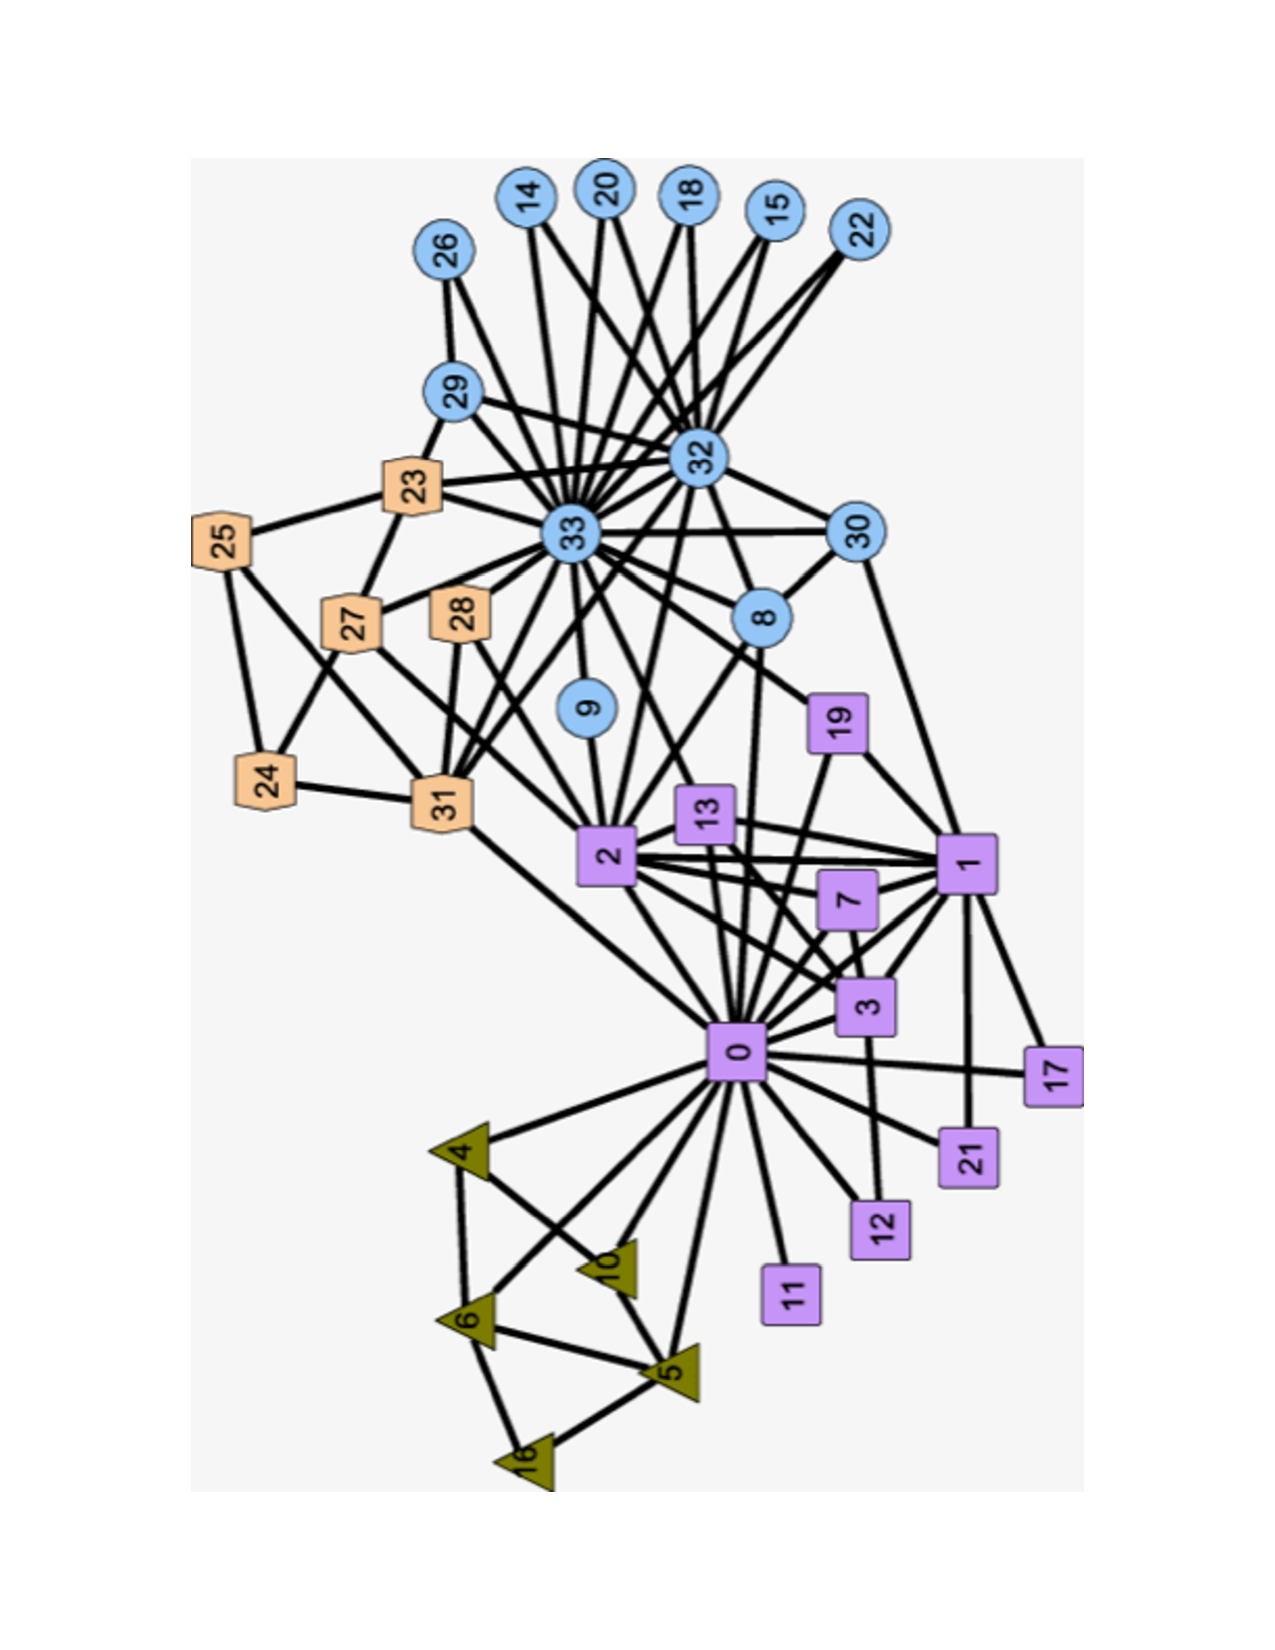
\includegraphics[width=.8\linewidth,angle=270]{Kempton/zkk.pdf}
\caption{Karate}
\end{subfigure}
\end{figure}
\end{center}
}

%\frame{\frametitle{Computational Results}
%\begin{center}
%%\begin{tikzpicture}
%%\draw (-1,-1)node[minimum size=2mm]{}--(-1,1)node[minimum size=2mm]{}--(1,1)node[minimum size=2mm]{}--(1,-1)node[minimum size=2mm]{}--(-1,-1)node[minimum size=2mm]{};
%%\draw (0,2)node[minimum size=2mm]{}--(1,1)node[minimum size=2mm]{};
%%\draw (-1,1)node[minimum size=2mm]{}--(0,2)node[minimum size=2mm]{};
%%\draw (1.1,-1)node[fill=none,right]{5};
%%\draw (-1.1,-1)node[fill=none,left]{4};
%%\draw (-1.1,1)node[fill=none,left]{2};
%%\draw (1.1,1)node[fill=none,right]{3};
%%\draw (0,2.1)node[fill=none,above]{1};
%%\node[fill=none] at (0,-3) {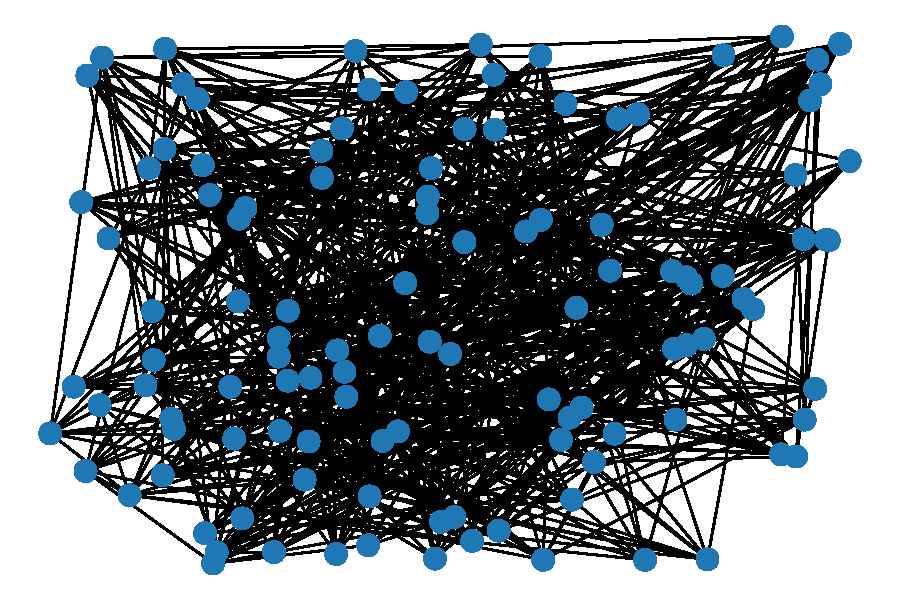
\includegraphics[scale=.3]{Kempton/football.pdf}};
%%\end{tikzpicture}
%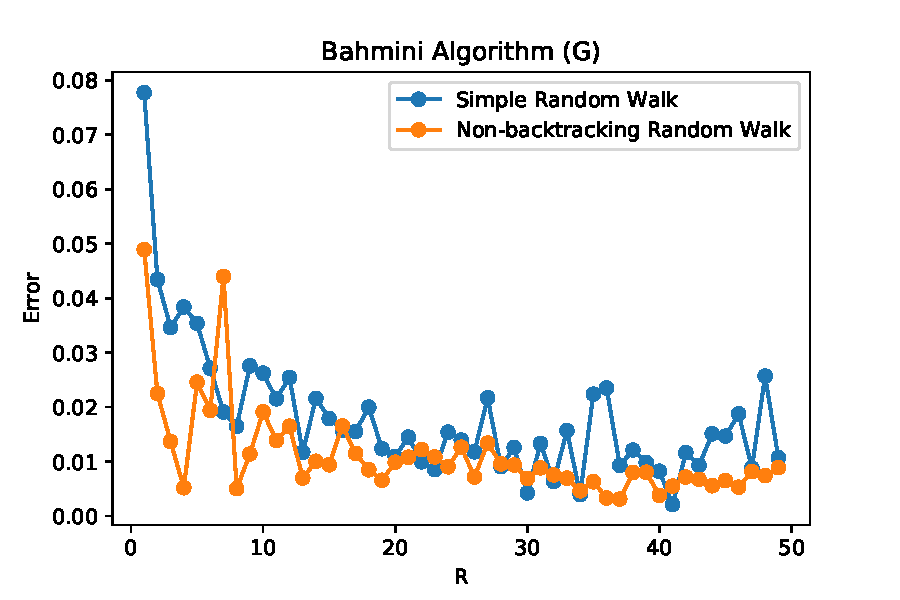
\includegraphics[width=.5\textwidth]{Kempton/bahmini_g.pdf}
%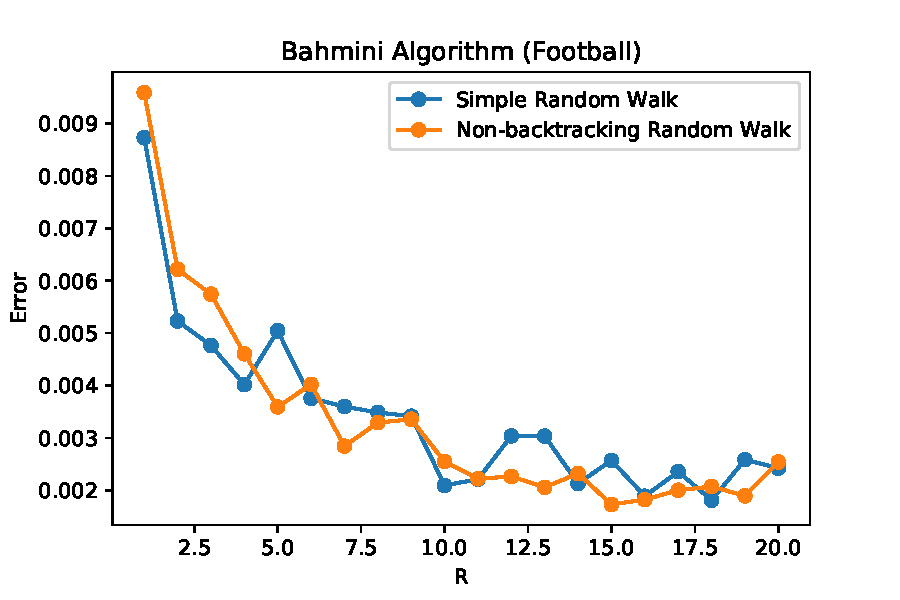
\includegraphics[width=.5\textwidth]{Kempton/bahmini_football.pdf}
%\end{center}
%}

\frame{\frametitle{Computational Results}
\[y=Cx^{-\alpha}\]
\begin{figure}
\centering
\begin{subfigure}[height=2in]{.5\textwidth}
  \centering
  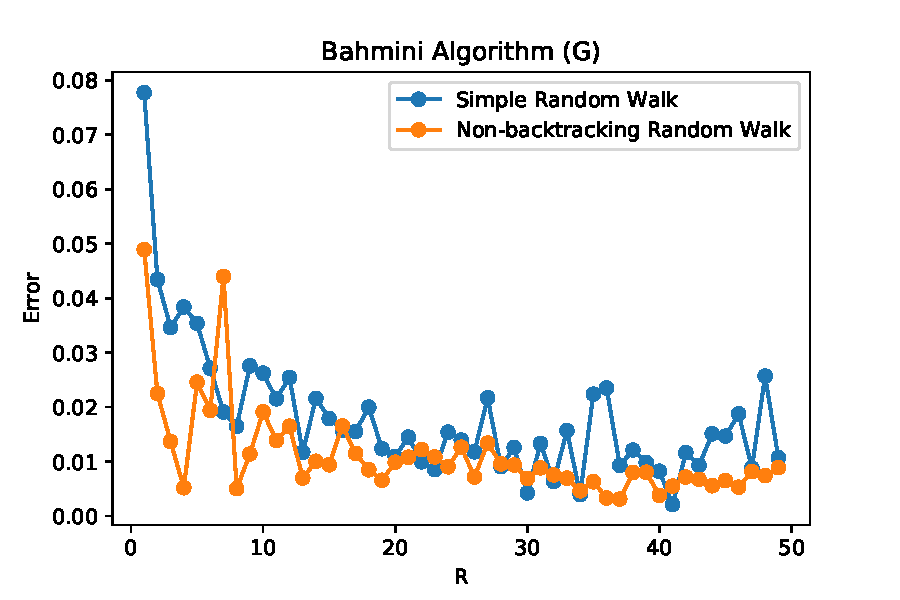
\includegraphics[width=.8\linewidth]{Kempton/bahmini_g.pdf}
  \caption{Simple Example}
  \label{fig:sub1}
\end{subfigure}%
\begin{subfigure}[height=2in]{.5\textwidth}
  \centering
  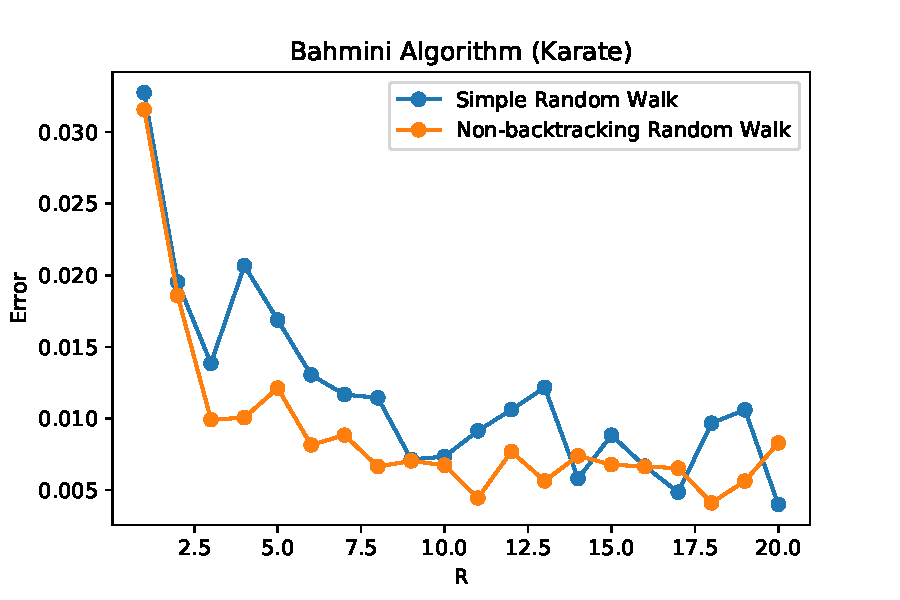
\includegraphics[width=.8\linewidth]{Kempton/bahmini_karate.pdf}
  \caption{Karate}
  \label{fig:sub2}
\end{subfigure}
%\begin{subfigure}[height=2in]{.5\textwidth}
%  \centering
%  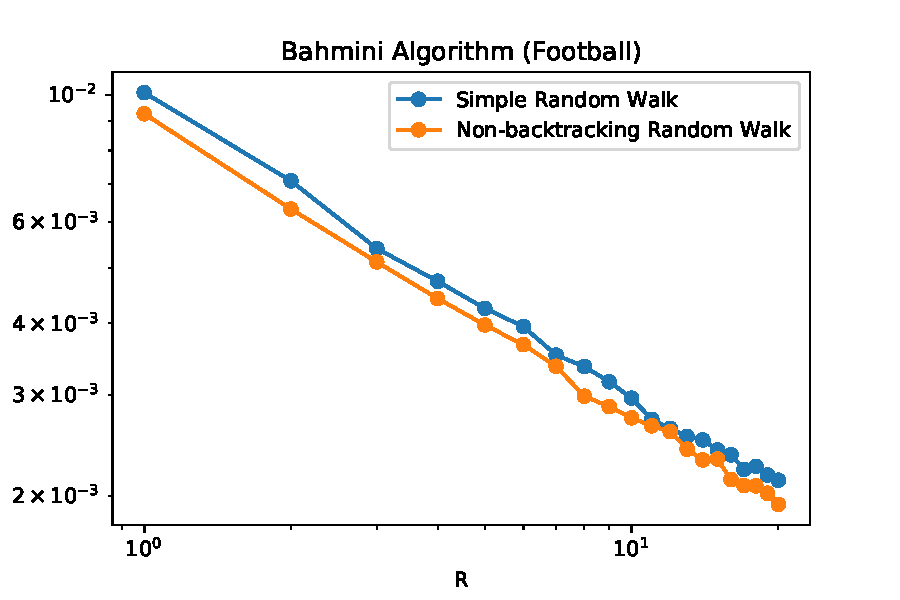
\includegraphics[width=.4\linewidth]{Kempton/power_law_football.pdf}
%  \caption{Football}
%  \label{fig:sub2}
%\end{subfigure}
\label{fig:test}
\end{figure}
}

\frame{\frametitle{Computational Results}
\begin{figure}
\centering
\begin{subfigure}[height=2in]{.5\textwidth}
  \centering
  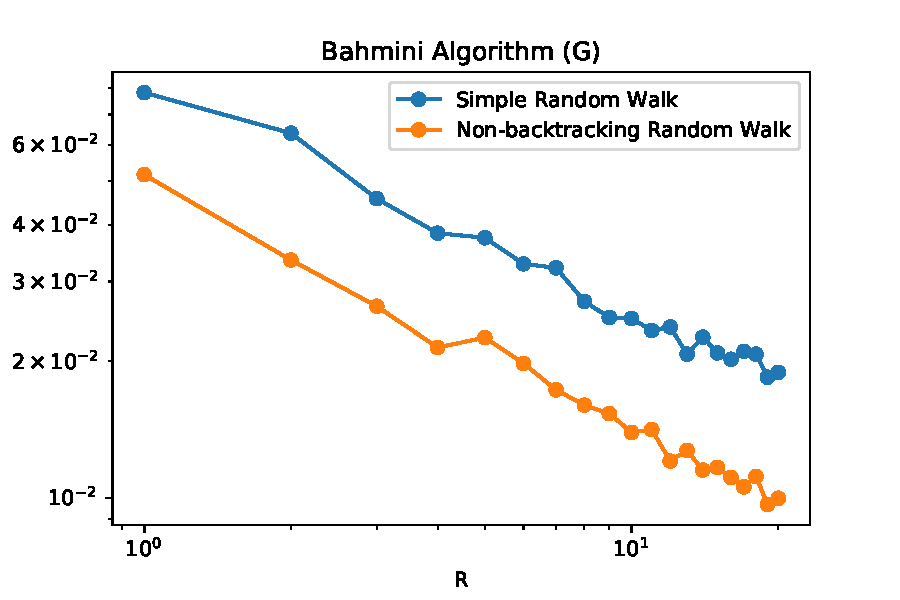
\includegraphics[width=.8\linewidth]{Kempton/power_law_g.pdf}
  \caption{\centering SRW: $\alpha=.54$, NBRW: $\alpha=.56$}
  \label{fig:sub1}
\end{subfigure}%
\begin{subfigure}[height=2in]{.5\textwidth}
  \centering
  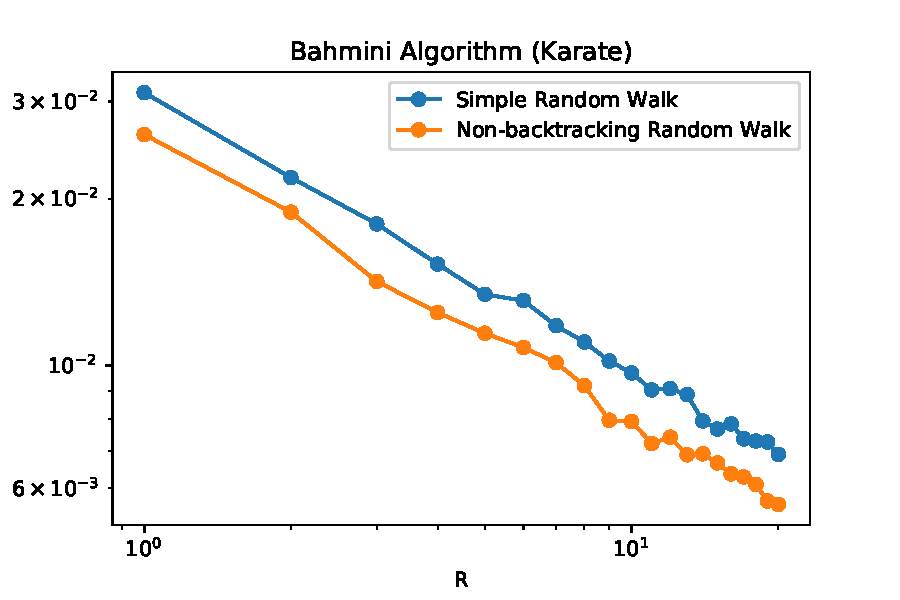
\includegraphics[width=.8\linewidth]{Kempton/power_law_karate.pdf}
  \caption{SRW: $\alpha=.49$, NBRW: $\alpha=.52$}
  \label{fig:sub2}
\end{subfigure}
%\begin{subfigure}[height=2in]{.5\textwidth}
%  \centering
%  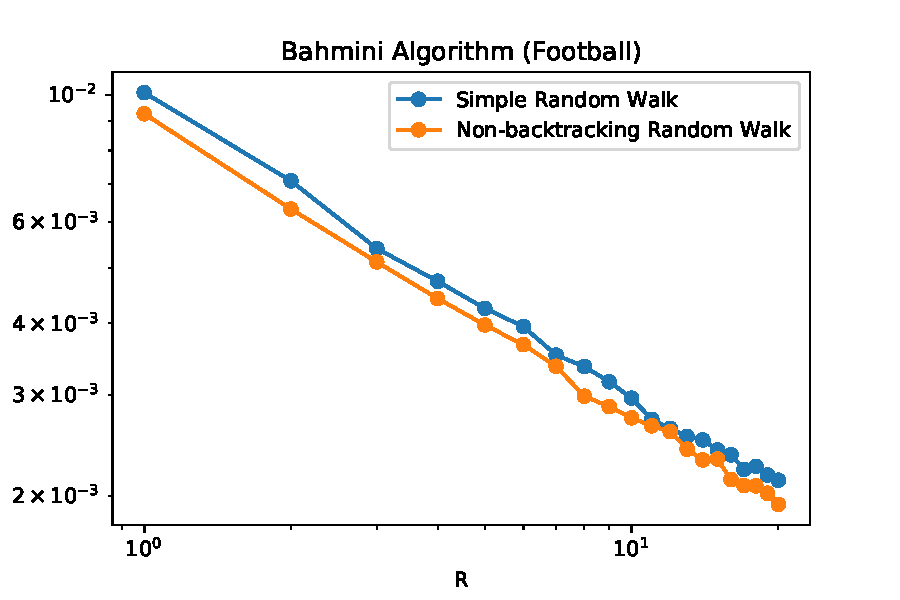
\includegraphics[width=.4\linewidth]{Kempton/power_law_football.pdf}
%  \caption{Football}
%  \label{fig:sub2}
%\end{subfigure}
\caption{Simple Example: $|C-C_{NB}|=.034$ \\ Karate: $|C-C_{NB}|=.0052$}
\label{fig:test}
\end{figure}
}


\frame{\frametitle{Conclusions}
\begin{center}
{\LARGE Thank you!}
\end{center}

}


\end{document}